\documentclass[twocolumn]{ctexart} 
\usepackage{tikz} 
\usepackage{amsmath} 
\usepackage{geometry} 
\usepackage{CJKfntef}
\geometry{a4paper, scale=0.75}
\begin{document} 
\subsection*{1-1} 
\noindent 
\textbf{解}: 

质点位移大小 
\begin{align*} 
|\Delta x|&=|x(4\ \mathrm{s})-x(0)|\ \mathrm{m} \\ 
&=|x(8\ \mathrm{s})-x(0)|\ \mathrm{m} \\ 
&=8\ \mathrm{m}. 
\end{align*} 


质点速度 
$$v=\frac{\mathrm{d}x}{\mathrm{d}t}=(6-2t)\ \mathrm{m/s},$$ 

令$v=0$, 解得$t=3\ \mathrm{s}$. 

质点在$t=3\ \mathrm{s}$时反转运动方向,总路程 
\begin{align*} 
s&=(|x(3\ \mathrm{s})-x(0)|+|x(4\ \mathrm{s})-x(3\ \mathrm{s})|)\ \mathrm{s}\\ 
&=(|9-0|+|8-9|)\ \mathrm{m}\\ 
&=10\ \mathrm{m}. 
\end{align*} 

\subsection*{1-2} 
\noindent 
\textbf{解:} 

由 
$$\left\{ 
\begin{array}{ll} 
x=2t,\\ 
y=12-2t^2\\ 
\end{array} 
\right. 
$$ 

得运动轨迹方程为 
$$x^2+2y=24,$$ 


质点坐标$$\vec{x}=(2t\hat{\mathbf{i}}+(12-2t^2)\hat{\mathbf{j}} )\ \mathrm{m},$$ 

速度和加速度矢量分别为 
\begin{align*} 
&\vec{v}=\frac{\mathrm{d}\vec{x}}{\mathrm{d}t}=(2\hat{\mathbf{i}}-4t\hat{\mathbf{j}})\ \mathrm{m/s},\\ 
&\vec{a}=\frac{\mathrm{d}\vec{v}}{\mathrm{d}t}=(-4\hat{\mathbf{j}})\ \mathrm{m/s^2}. 
\end{align*} 
\subsection*{1-3} 
\noindent 
\textbf{解:} 

设质点的速度为$v$, 质点在4.5 s时的位置 
$$x(4.5\ \mathrm{s})=\int_{0}^{4.5\ \mathrm{s}}v\mathrm{d}t.$$ 

由图象可得积分值 
\begin{align*} 
\int_{0}^{4.5\ \mathrm{s}}v\mathrm{d}t&=(\frac{(1+2.5)\times 2}{2}-\frac{(1+2)\times 1}{2})\ \mathrm{m}\\ 
&=2\ \mathrm{m}. 
\end{align*} 

故$t=4.5\ \mathrm{s}$时质点位于$x=2\ \mathrm{m}$处. 

\subsection*{1-4} 
\noindent 
\textbf{解:} 

\begin{align} 
&a=\frac{\mathrm{d}v}{\mathrm{d}t}=\frac{\mathrm{d}v}{\mathrm{d}x}\cdot\frac{\mathrm{d}x}{\mathrm{d}t}=v\frac{\mathrm{d}v}{\mathrm{d}x}\\ 
&a=(3+9x^2)\ \mathrm{m/s^2} 
\end{align} 

由(1)(2)得 
$$v\mathrm{d}v=(3+9x^2)\mathrm{d}x.$$ 

利用$\left.v\right|_{t=0}=0$积分: 
$$\int_{0}^{v}v\mathrm{d}v=\int_{0}^{x}(3+9x^2)\mathrm{d}x,$$ 

得 
$$\frac{v^2}{2}=3x+3x^3.$$ 

取合理解 
$$v=\sqrt{6x+6x^3}\ \mathrm{m/s}.$$ 
\subsection*{1-5} 
\noindent 
\textbf{解:} 

\subsubsection*{(1)} 
$x(2\ \mathrm{s})=-7\ \mathrm{m},x(1\ \mathrm{s})=2.5\ \mathrm{m}.$ 平均速度 
$$\bar{v_{12}}=\frac{x(2\ \mathrm{s})-x(1\ \mathrm{s})}{2\ \mathrm{s}-1\ \mathrm{s}}=-9.5\ \mathrm{m/s}.$$ 
\subsubsection*{(2)} 
\begin{align*} 
&v(t)=\frac{\mathrm{d}x}{\mathrm{d}t}=(4.5-6t^2)\ \mathrm{m/s},\\ 
&v(2\ \mathrm{s})=-19.5\ \mathrm{m/s}. 
\end{align*} 
\subsubsection*{(3)} 
令$v(t)=0$, 取合理解$\displaystyle{t=\frac{\sqrt{3}}{2}\ \mathrm{s}<1\ \mathrm{s}}$,因此在第2秒内质点向同一方向运动. 

质点运动的路程 
$$s=|x(2\ \mathrm{s})-x(1\ \mathrm{s})|=9.5\ \mathrm{m}.$$ 

\subsection*{1-6} 
\noindent 
\textbf{解:} 

由 
\begin{align*} 
&\frac{\mathrm{d}v}{\mathrm{d}t}=-kv^2,\\ 
&\frac{\mathrm{d}v}{\mathrm{d}t}=v\frac{\mathrm{d}v}{\mathrm{d}x} 
\end{align*} 

得$\displaystyle{\frac{\mathrm{d}v}{v}=-k\mathrm{d}x}$,积分 
$$\int_{v_0}^{v}\frac{\mathrm{d}v}{v}=\int_{0}^{x}-k\mathrm{d}x$$ 

得$\displaystyle{\ln\frac{v}{v_0}=-kx}$, 即 
$$v=v_0 \mathrm{e}^{-kx}.$$ 
\subsection*{1-7} 
\noindent 
\textbf{解:} 

\subsubsection*{(1)} 
$$\vec{v}=\frac{\mathrm{d}\vec{r}}{\mathrm{d}t}=-\omega a\sin\omega t\hat{\mathbf{i}}+\omega b\cos\omega t\hat{\mathbf{j}}.$$ 
\subsubsection*{(2)} 
$$ 
\left\{ 
\begin{array}{ll} 
x=a\cos\omega t,\\ 
y=b\sin\omega t\\ 
\end{array} 
\right.$$ 

消去$t$得椭圆方程 
$$\frac{x^2}{a^2}+\frac{y^2}{b^2}=1.$$ 
\subsubsection*{(3)} 
$\displaystyle{\vec{a}=\frac{\mathrm{d}\vec{v}}{\mathrm{d}t}=-{\omega}^2\vec{x}}$, 即$\vec{a}$和$\vec{x}$反向. 故$\vec{a}$指向椭圆中心. 
\subsection*{1-8} 
\noindent 
\textbf{解:} 

由几何关系, 

$$\frac{h}{H}=\frac{x-s}{x}.$$ 

即$hx=Hx-Hs$, 两侧对$t$求导得 
$$h\frac{\mathrm{d}x}{\mathrm{d}t}=H\frac{\mathrm{d}x}{\mathrm{d}t}-H\frac{\mathrm{d}s}{\mathrm{d}t}.$$ 

代入$\displaystyle{\frac{\mathrm{d}s}{\mathrm{d}t}=v_0}$得 
$$\frac{\mathrm{d}x}{\mathrm{d}t}=\frac{Hv_0}{H-h},$$ 

此即影子端点移动的速度. 
\subsection*{1-9} 
\noindent 
\textbf{解:} 

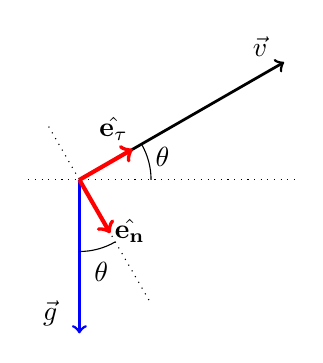
\begin{tikzpicture}[scale=1.3] 
\draw[line width=1pt][->] (0,0)--(2, 1.15); 
\draw[line width=1pt, color=blue][->] (0,0)--(0,-1.5); 
\node[right] at(1.6, 1.3) {$\vec{v}$}; 
\node[right] at(-0.45, -1.3) {$\vec{g}$}; 
\draw[dotted] (-0.5,0)--(2.1,0); 
\draw[dotted] (-0.3, 0.52)--(0.7,-1.21); 
\draw (0, -0.7) arc (270:300:0.7); 
\draw (0.7, 0) arc (0:30:0.7); 
\node[right] at(0.65, 0.22) {$\theta$}; 
\node[right] at(0.05, -0.9) {$\theta$}; 
\draw[line width=1.5pt, color=red][->] (0,0)--(0.52, 0.3); 
\draw[line width=1.5pt, color=red][->] (0,0)--(0.3, -0.52); 
\node[right] at(0.1, 0.5) {$\hat{\mathbf{e_{\tau}}}$}; 
\node[right] at(0.25, -0.5) {$\hat{\mathbf{e_n}}$}; 
\end{tikzpicture} 

$\vec{v}$的方向为运动轨迹切线的方向, 如图建立自然坐标系, 则有 
\begin{align*} 
&\left|a_{\tau}\right|=\left|-g\sin\theta\right|=g\sin\theta,\\ 
&\left|a_n\right|=\left|g\cos\theta\right|=g\cos\theta. 
\end{align*} 
\subsection*{1-10} 
\noindent 
\textbf{解:} 

在极坐标系中讨论问题. 由于质点做圆周运动, 故法向加速度只有向心加速度部分, 质点在轴向运动的加速度为0, 切向加速度只有角速度变化对应的加速度, 而没有轴向速度变化对应的加速度. 

\setcounter{equation}{0} 
\begin{align} 
&a_\tau=\left|r\ddot{\theta}\right|\\ 
&a_n=\left|-r{\dot{\theta}}^2\right|\\ 
&r=R\\ 
&s=bt-\frac{1}{2}ct^2\\ 
&s=R\theta 
\end{align} 

由(1)至(5)解得$\displaystyle{a_\tau=c,a_n=\frac{1}{R}\left(b-ct\right)^2}$. 

取$a_\tau=a_n$得 
$$t_1=\frac{b}{c}+\sqrt{\frac{R}{c}},t_2=\frac{b}{c}-\sqrt{\frac{R}{c}}.$$ 

均为合理解. 
\subsection*{1-11} 
\noindent 
\textbf{解:} 
\subsubsection*{(1)} 
任意时刻质点的切向加速度 
\begin{align*} 
a_\tau&=\frac{\mathrm{d}^2s}{\mathrm{d}t^2}\\ 
&=\frac{\mathrm{d}^2}{\mathrm{d}t^2}\left(v_0t-\frac{1}{2}bt^2\right)\\ 
&=-b. 
\end{align*} 

法向加速度 
\begin{align*} 
a_n&=\frac{v^2}{R}\\ 
&=\frac{1}{R}\left(\frac{\mathrm{d}s}{\mathrm{d}t}\right)^2\\ 
&=\frac{1}{R}\left(v_0-bt\right)^2. 
\end{align*} 

在自然坐标系中, 质点的加速度为 
$$\vec{a}=-b\hat{\mathbf{e_\tau}}+\frac{1}{R}\left(v_0-bt\right)^2\hat{\mathbf{e_n}}.$$ 

其中$\hat{\mathbf{e_\tau}}$在运动轨迹上定向为质点在圆周上初始的运动方向, $\hat{\mathbf{e_n}}$指向圆心. 
\subsubsection*{(2)} 
质点的加速度大小 
\begin{align*} 
a&=\left|\vec{a}\right|\\ 
&=\sqrt{\left(-b\right)^2+{\left[\frac{1}{R}\left(v_0-bt\right)^2\right]}^2}\\  
\end{align*} 

令$a=b$解得$\displaystyle{t=\frac{v_0}{b}}$.

当$\displaystyle{t=\frac{v_0}{b}}$时, 质点的加速度大小为$b$. 
\subsection*{1-12} 
\noindent 
\textbf{解:} 

轮船B相对岸上的速度$\vec{v'}$和小船A相对轮船B的速度$\vec{v_r}$分别为 
\begin{align*} 
&\vec{v'}=25\hat{\mathbf{i}}\ \mathrm{km/h},\\ 
&\vec{v_r}=40\hat{\mathbf{j}}\ \mathrm{km/h}. 
\end{align*} 

设小船相对岸上的速度为$\vec{v}$, 由伽利略坐标变换求导可得 
$$\vec{v'}=\vec{v}-\vec{v_r},$$ 

即 
\begin{align*} 
\vec{v}&=\vec{v_r}+\vec{v'}\\ 
&=(25\hat{\mathbf{i}}+40\hat{\mathbf{j}})\ \mathrm{km/h}. 
\end{align*} 
\subsection*{1-13} 
\noindent 
\textbf{解:} 

在车中观察, 水平方向上雨滴以$12\ \mathrm{m/s}$的速度向北运动, 竖直方向上水滴以$28\ \mathrm{m/s}$的速度向下运动,水滴的速度大小为 
$$v=\sqrt{12^2+28^2}\ \mathrm{m/s}=4\sqrt{58}\ \mathrm{m/s}=30.46\ \mathrm{m/s}.$$ 

速度与竖直方向夹角$$\theta=\arctan(12/28)=23.2^{\circ},$$

方向向北.
\subsection*{1-14} 
\noindent 
\textbf{解:} 

无论在汽车还是大地参考系中, 雨滴的竖直速度都是一样的. 要使雨滴\CJKunderdot{\textbf{刚好}}不淋湿物体, 雨滴在汽车参考系中的速度与竖直方向夹角要达到$\alpha=\arctan(l/h)$. 设雨滴的竖直速度为$v_v=v_e\cos\theta$, 在汽车参考系中的水平速率为$v'_f$, 在大地参考系中的水平速率为$v_f$. 则$v_f=v_2\sin\theta$, $v_1=v_f+v'_f$, 结合$v'_f/v_v=\tan\alpha$可得 
$$v_1=v_2\left(\frac{l}{h}\cos\theta+\sin\theta\right).$$ 
\subsection*{1-15} 
\noindent 
\textbf{解:} 
\setcounter{equation}{0} 

以船的出发点为原点, 水流方向为$x$方向, 垂直河岸指向河心为$y$方向建立直角坐标系. 

当$0\leq y\leq L/2$时, 河水流速 
\begin{align} 
v_r=\frac{2v_0}{L}y. 
\end{align} 

由于小船相对水流垂直运动, 故小船的水平速度可认为是河水流速. 
\begin{align} 
&\frac{\mathrm{d}x}{\mathrm{d}t}=v_r 
\end{align} 

小船向河心运动时, 有
\begin{align} 
&\frac{\mathrm{d}y}{\mathrm{d}t}=u\\ 
&\left.x\right|_{t=0}=0\\ 
&\left.y\right|_{t=0}=0 
\end{align} 

得到积分 
$$\int_{0}^{y}2v_0y\mathrm{d}y=\int_{0}^{x}uL\mathrm{d}x,$$ 

即 
$$v_0y^2=uLx,$$ 

令$\displaystyle{y=\frac{L}{4}}$可得掉头点坐标$\displaystyle{\left(\frac{v_0L}{16u}, \frac{L}{4}\right)}$. 则船驶向对岸的轨迹为 
$$v_0y^2=uLx,0\leq x\leq \frac{L}{4}.$$ 

由返回时$y$坐标对时间的均匀性得船在返回过程中沿$x$方向运动的距离为$\displaystyle{\left(\frac{u}{u/2}\right)\frac{v_0L}{16u}=\frac{v_0L}{8u}}$.

全过程横向位移
$$\Delta x=\frac{v_0L}{8u}+\frac{v_0L}{16u}=\frac{3v_0L}{16u}.$$
\end{document}